\chapter{Theory and implementation}
\section{The inverse problem}
Full waveform inversion (FWI) aims to minimise the misfit between modeled and observed data to find a subsurface model $\textbf m$ which explains the observed data optimally. IFOS3D uses the $L_2$-norm based misfit function $E$ given by 
\begin{equation}E(\textbf m)=\frac{1}{2}\sum_{s}\int_0^T dt \sum_{r}\delta u_i(\textbf x_s,\textbf x_r,t)^2, \label{eq:L2}\end{equation}
with the $i$-th component of the displacement residual $\delta u_i=u_i-u_{i,obs}$ at source position $\textbf x_s$ and receiver position $\textbf x_r$. $\textbf u_{obs}$ denotes the observed data, whereas $\textbf u$ denotes the modelled data. The squared residuals are summed up over all sources $s$ and receivers $r$ and integrated over time $t$ for the full record length $T$. In this and the following equations we use the Einstein notation to sum up over double indices.
\subsection*{The gradient methods}
A conjugate gradient approach is applied to solve this optimisation problem. Gradient methods are local inversion methods, which iteratively minimise the misfit by updating the model in the direction of the steepest descent of $E$. The model in iteration $k$ is updated by 
\begin{equation} \textbf m_{k+1}=\textbf m_k-\alpha_k\textbf p_k \hspace{0.4cm}\text{with} \hspace{0.4cm}\textbf p_k=\textbf P\nabla_mE_k. \label{equ:update1} \end{equation}
Hereby $\nabla_mE_k$ is the gradient of the misfit function, $\textbf P$ is a preconditioning operator, which mitigates amplitude effects in the gradient, and $\alpha_k$ is the step length. Gradient directions in FWI can be implemented very efficiently with the adjoint approach \citep[e.g.][]{Tar84, Mor87} and these methods are thus applicable even for larger problem sizes. Note however, that the misfit function in FWI is generally very rough and contains local minima. In order to reach the global minimum with this local inversion method, a good starting model and the application of inversion strategies, like frequency filtering are essential. \\
The use of the conjugate gradient $\textbf c_k$ compared to the general gradient $\nabla_mE_k$ can improve the convergence. The conjugate gradient direction $\textbf c_k$ in iteration $k$ is given by 
\begin{equation}\textbf c_k=\textbf P\nabla_m E_k+\beta_k\textbf c_{k-1}. \label{equ:conjgrad1} \end{equation} This stabilises the inversion by adding some part of the previous gradient.  The scalar $\beta$ is estimated with the Polak-Ribi\'{e}re method as 
\begin{equation}\beta_k=\frac{\textbf p_k^T(\textbf p_k-\textbf p_{k-1})}{||p_{k-1}||^2}\hspace{0.15cm} \text{for} \hspace{0.15cm}\beta_k>0; \hspace{0.5cm}\beta_k=0 \hspace{0.15cm}\text{for} \hspace{0.15cm}\beta_k<0.\label{equ:beta}\end{equation}
The distinction of cases ensures, that the model is updated in the decent direction of the misfit function. The new model is then estimated as
\begin{equation}\textbf m_{k+1}=\textbf m_k-\alpha_k\textbf c_k. \label{equ:conjgrad2} \end{equation}

\section{Forward modeling with SOFI3D}
Before explaining the inversion process, we will shortly describe the solution of the forward problem. 3D  elastic FWI requires a forward solver, which accurately simulates seismic wave propagation in the elastic media. Otherwise artefacts and deviations in the inversion result can be caused by fitting modelling errors in the wavefield. Additionally, a computationally efficient forward solver is required, because the inversion process is characterised by a high number of forward modellings and the FWI runtime is thus mainly influenced by the runtime spend for wavefield modelling. \\
``IFOS3D'' uses the elastic version of the time-domain finite-difference solver ``SOFI3D'' \citep{boh02} for wavefield modelling, which very efficiently and fast solves the 3D elastic wave equation. The code discretizes the velocity stress formulation of the elastic wave equation on a staggered grid \citep{Vir86, Lev88}. It is able to accurately model wave propagation in 3D complex media. A viscoelastic version of SOFI3D exits, but was not tested for FWI yet. In the following, I will give a short overview of SOFI3D and its characteristics, but refer to the SOFI3D manual for a more detailed description of its theory, implementation and performance.\\
Wave propagation can be described in the velocity-stress formulation. This formulation uses the particle velocity $\textbf v=\partial\textbf u/\partial t$ as wavefield parameter. For the elastic isotropic medium wave propagation due to a force $\textbf f$ can then be described as first order differential equations:
\begin{equation}
 \begin{split}
  \rho\frac{\partial v_i}{\partial t}=f_i+\frac{\partial\tau_{ij}}{\partial x_j},\\
\frac{\partial\tau_{ij}}{\partial t}-\lambda\frac{\partial\Theta}{\partial t}\delta_{ij}+2\mu\frac{\partial\epsilon_{ij}}{\partial t}=0,\\
\frac{\partial\epsilon_{ij}}{\partial t}=\frac{1}{2}\left (\frac{\partial v_i}{\partial x_j}+\frac{\partial v_j}{\partial x_i}\right ).
 \end{split}\label{equ:wave_equvel}
\end{equation}
The elastic medium is described by the density $\rho$ and the Lam\'e parameters $\lambda$ and $\mu$. $\tau_{ij}$ denotes the elements of the stress tensor and $\epsilon_{ij}$ denotes the elements of the strain tensor. The trace of the stress tensor is given by $\Theta$.
\subsection{Finite difference modeling}\label{sec:FDmodeling}
For the simulations of 3D elastic wave propagation these equations are approximated by finite differences (FD). For the calculation of partial derivatives, the wavefield parameters and model parameters are discretised on a staggered-grid system \citep{Vir86, Lev88}. The 3D staggered-grid system is sketched in Figure~\ref{fig:stag_grid}. We use a Cartesian grid (x,y,z)=(i,j,k). The model parameters $\lambda$, $\mu$ and $\rho$ and the diagonal stress components $\sigma_{ii}$ are localised on the full grid points, whereas velocities and off-diagonal stress components are calculated on a grid which is half a grid point shifted to the original system. Compared to a conventional Cartesian grid, the staggered grid enables a larger grid spacing for the same level of accuracy.\\
\begin{figure}
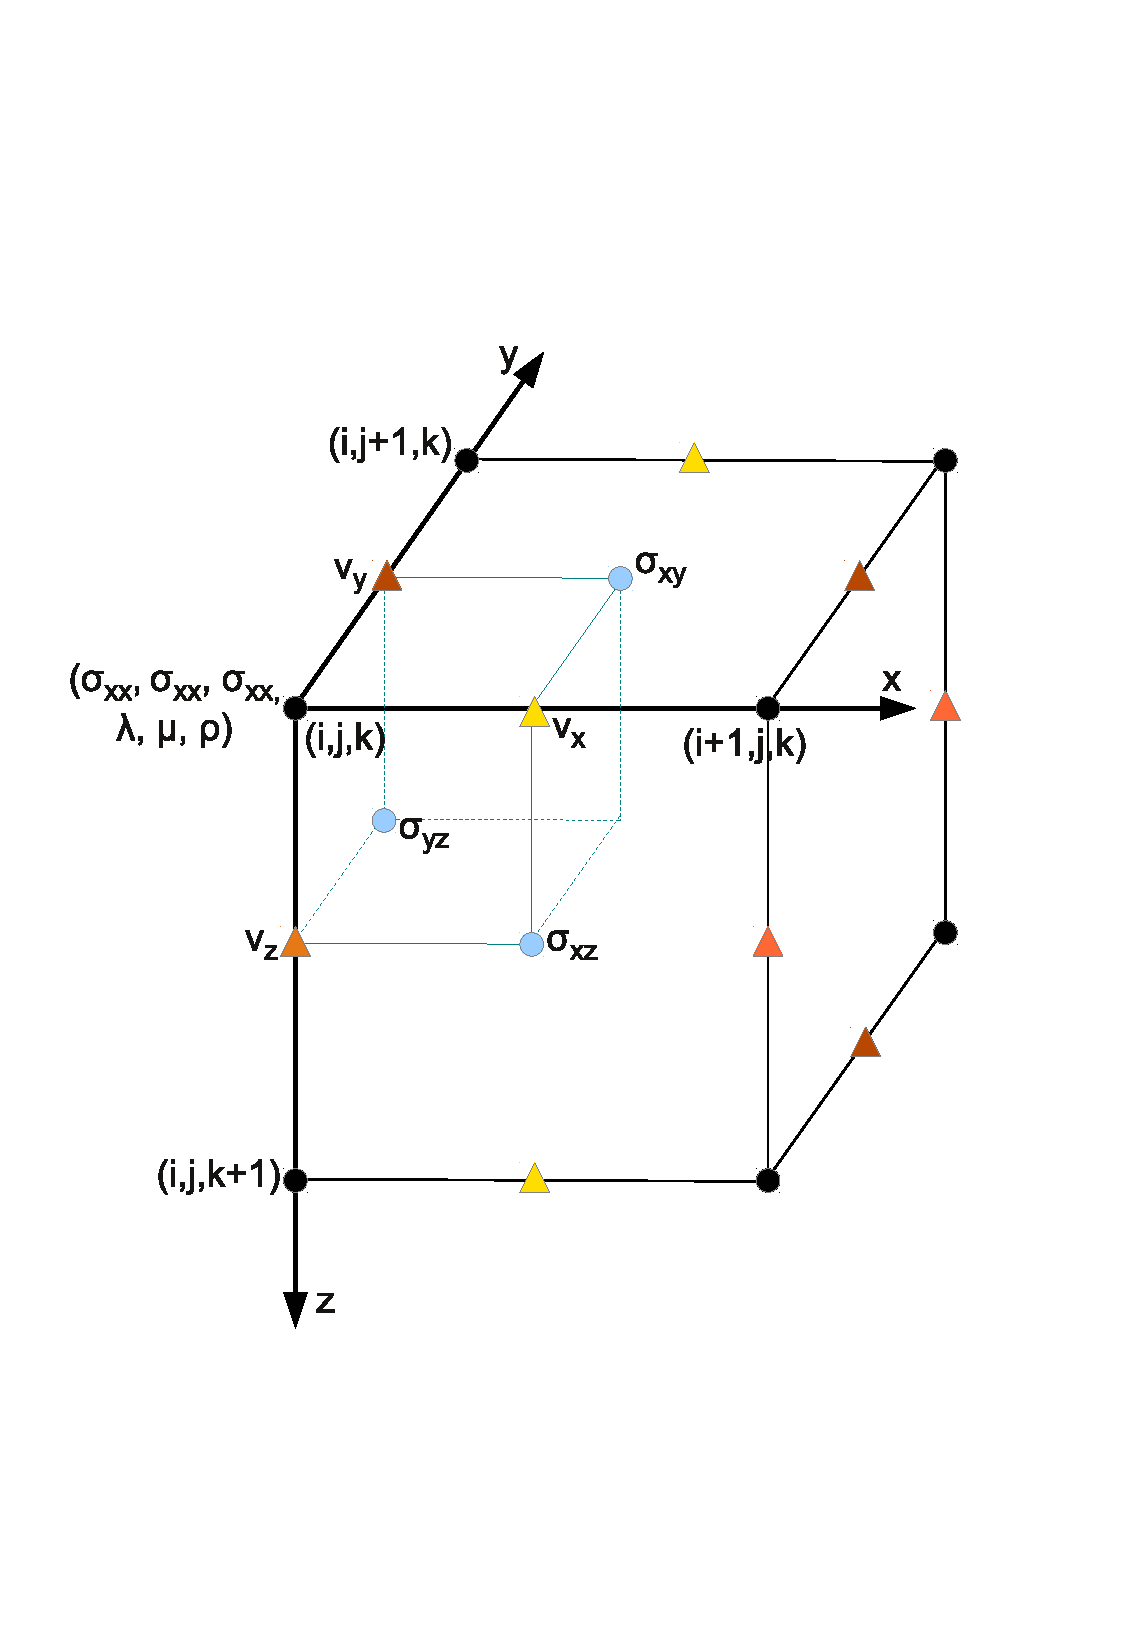
\includegraphics[width=0.7\textwidth]{fig/staggered_grid}
\caption[Staggered grid system]{Staggered-grid coordinate system used for 3D FD modelling in SOFI3D}\label{fig:stag_grid}
\end{figure}
The derivatives are approximated by centered finite differences. The easiest finite-differences are of second order, where the two adjacent grid points with a grid space $dh$ are used to calculate the derivative between these grid points as follows
\begin{equation}
 \frac{\partial f(x)}{\partial x}|_{i+1/2}\approx \frac{f[i+1]-f[i]}{dh}
\end{equation}
 The consideration of additional grid points in higher order schemes can increase the accuracy and thus enable a larger grid spacing. However, it needs to be considered, that the number of operations increases and the number of parameters which are interchanged during MPI communication rises. Additionally, high order finite-difference operators can cause problems in case of large discontinuities, like tunnels. The SOFI code uses second order temporal and second to 12th order spatial finite difference operators, which can be chosen according to the problem.\\
To solve the system of equations~\ref{equ:wave_equvel} two steps are performed for each time step: 
\begin{itemize}
 \item velocity updates are calculated using spatial stress derivatives and are added to the previous velocity values
\item stress value updates are calculated using spatial velocity derivatives and Hook's law and are summed to the previous stress values
\end{itemize}
Hereby the summation of the update values over all time steps accounts for the time derivatives of velocity and stress values. 
\subsection{Additional charactersistics of SOFI3D}\label{sec:SOFI3Dcharacter}
\subsubsection*{Boundary conditions}
There are two ways to avoid arteficial reflections from model boundaries in SOFI3D. The first exponentially damps waves within a boundary zone surrounding the model by multiplying the amplitudes with an exponentially decaying factor \citep{Cer85}. At least 30 gridpoints thickness at boundary zones is required. The second method is the implementation of convolutional perfectly matched layers (C-PMLs) \citep{Ber94,Kom07}. This method can offer a much better performance compared to the  conventional exponential damping and a boundary zone of 10 gridpoints thickness is generally sufficient. However, in case of strong contrasts and heterogeneities at the model boundary instabilities can be caused.
\subsubsection*{The free surface}
At the free surface, the vertical stress components $\sigma_{xz}$, $\sigma_{yz}$ and  $\sigma_{zz}$ are zero. A planar free surface is implemented implicitely in SOFI3D with the mirroring technique described by \cite{Lev88}.
\subsubsection*{Grid dispersion and stability} 
To mitigate numerical dispersion and grid anisotropy of the wavefield the grid spacing must be chosen sufficiently small. For a fourth-order spatial and second-order temporal scheme the criterion 
\begin{equation}
 dh < \frac{\lambda_{min}}{6}=\frac{v_{min}}{6f_{max}} \label{equ:grid_disp}
\end{equation}
ensures a wavefield error of less than 5\% \citep{boh02}. It depends on the minimum wavelength $\lambda_{min}$, defined by the minimum velocity $v_{min}$ and the maximum frequency $f_{max}$.  Higher order FD-operators enable a larger grid spacing.\\
In order to ensure stability of the simulation, the temporal spacing must satisfy the Courant-Friedrichs-Levy (CFL) stability criterion \citep{Cou67}. It is related to the maximum velocity $v_{max}$ and is given by
\begin{equation}
 dt<=\frac{dh}{h\sqrt{3}v_{max}}.
\end{equation}
The constant factor $h$ amounts to $\frac{7}{6}$ for a Taylor operator of fourth order. For different FD orders and Holberg coefficients we refer to the SOFI manual.
\subsubsection*{Viscoelasticity}
A viscoelastic version of SOFI3D exists. For its implementation we refer to \cite{boh02}. So far we only employed the elastic version of SOFI3D for IFOS3D. However, it would be possible to include the viscoelastic update functions. This enables the use of viscoelasticity as passive parameter in the inversion process. This could already be successfully tested for the 2D elastic FWI with IFOS2D.	
\section{The inversion process - overview}
Figure \ref{fig:workflow} explains the different steps, which are performed within each iteration of the conjugate gradient algorithm in IFOS3D. Each iteration can be divided into three parts. First, the misfit gradient $\Delta E_k(\textbf m)$ for each shot and model parameter ($\textbf m$) is calculated. Second, to calculate the search direction ($\textbf{c}_k$), the misfit is summed up over all shots, preconditioned and the conjugate gradient $\textbf c_k$ is calculated. Third, a step length estimation is performed, which determines the total size of the update. IFOS3D additionally enables the calculation of a diagonal Hessian approximation and the use of the L-BFGS sheme, which will be described in section \ref{sec:hess} and \ref{sec:lbfgs}, respectively.\\
The conjugate gradient method is realised with a time-frequency approach \citep{Sir08}. Wavefield modeling is performed in time domain using the finite difference solver SOFI, whereas the gradient is calculated in frequency domain. A discrete Fourier transformation on the fly is applied to calculate the frequency domain wavefields. The main advantage of the frequency domain inversion is the possibility to calculate the gradient only for few discrete frequencies \citep[e.g.][]{Pra99,Sir04,Bro09}. This results in an enormous reduction of storage costs compared to a time domain inversion, which generally requires the storage of the full forward field. The time-frequency approach additionally allows the use of the efficient and fast 3D time-domain FD forward solver. Thus, for 3D elastic FWI it is recommendable regarding computational performance. 
\begin{figure}[h!]
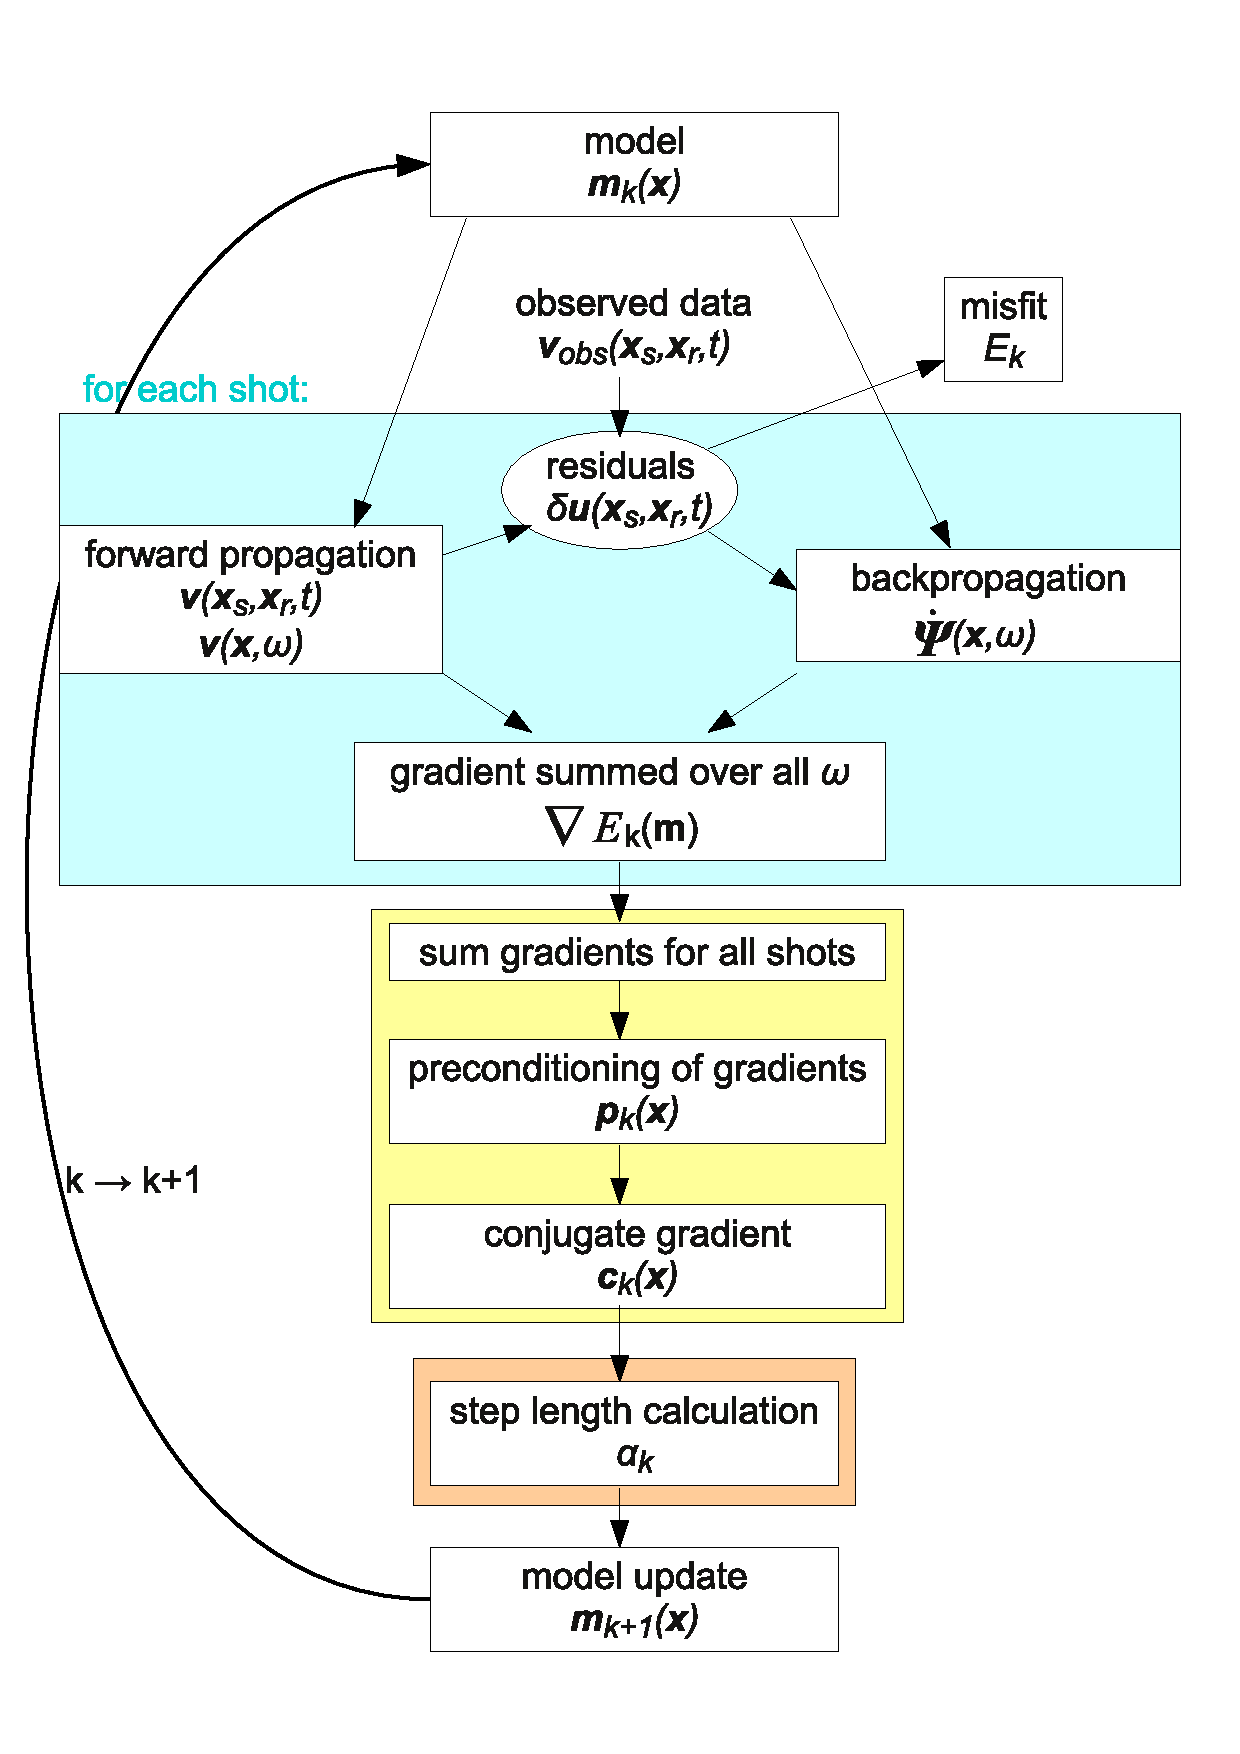
\includegraphics[width=0.9\textwidth]{fig/workflow}
\caption[IFOS3D workflow]{The workflow of IFOS3D shows the different steps performed during each iteration.}\label{fig:workflow}
\end{figure}

\section{Gradient calculation}\label{sec:grad_calc}
The misfit gradient is calculated with the adjoint method, which can be derived from perturbation theory \citep[e.g.][]{Tar84, Mor87}. The blue box of the workflow in Figure~\ref{fig:workflow} gives a sketch of its implementation and shows the gradient as multiplication of the forward wavefield and the conjugate adjoint wavefield. A detailed derivation of the gradient equations in IFOS3D is given by \cite{But15}. Here, we will only give a short overview about the employed equations and concentrate on the implementation.
\subsection{Extraction of monochromatic wavefields}
For the gradient calculation in frequency domain wavefield parameters of the forward and backpropagated wavefields are required for discrete frequencies. We follow the approach by \cite{Sir08} and use the discrete Fourier transformation
\begin{equation}\tilde{A}_i(\textbf x,\omega)=\sum_{l=0}^{nt}\exp(i\omega l\Delta t)A_i(\textbf x,l\Delta t)\Delta t, \label{equ:discFourier}  \end{equation}
 to extract the monochromatic wavefields, where $nt$ is the number of timesteps, $\Delta t$ the time sampling and $A_i$ a wavefield parameter. The discrete Fourier transformation is performed on the fly, summing up Fourier summands of $A_i$ in each time step. Therefore, no storage of the time domain wavefields at different time steps is required. Furthermore, the number of additional operations is low, as long as the transformation is only performed for few frequencies. Thus, the change from time to frequency domain can be achieved at low extra costs.
\subsection{Wavefield calculation}
In a first step, the forward-propagated wavefield for the model $\textbf m_k$ is simulated, which travels from source into medium. At each receiver position the seismograms $v(\textbf x_r,t)$ are stored. Additionally, by applying a discrete Fourier transformation (equation~\ref{equ:discFourier}), we calculate the particle velocities $\tilde v(\textbf x,\omega$), which are stored in memory for each discrete inversion frequency and at each grid point.\\
At each receiver position the time-reversed, residual displacement seismograms  $\delta u_i(\textbf x_r,T-t')$ are estimated. This residual is back-propagated from all receivers into the medium simultaneously. The corresponding backpropagated wavefield is defined as \begin{equation} \Psi_j(\textbf x,T-\tau)=\sum_{r}\int_0^T dt' G_{ji}(\textbf x,\tau;\textbf x_r,t')\delta u_i(\textbf x_r,T-t').\label{equ:psi}\end{equation} 
Hereby we use the same forward solver, which is based on the first-order wave-equation and therefore calculates the time derivative $\partial\Psi/\partial t=\dot\Psi$. For the backpropagation, the time line is reversed and we calculate wavefields starting from time $T$ backwards. Same as for the forward propagation, we extract the frequency wavefields $\tilde{\dot\Psi}(\textbf x,\omega)$ on the fly. These frequency wavefields are stored in memory for each frequency.
\subsection{Gradient equations in time and frequency domain}
Finally the gradients are calculated as multiplication of the forward and conjugate adjoint wavefields for each frequency and summed up over all frequencies. In the following the corresponding equations are described in more detail.\\
In time domain the misfit gradients for the elastic parameters $\lambda$, $\mu$ and $\rho$ can be estimated as zero-lag cross-correlation between forward and backpropagated wavefields as \citep[e.g.][]{Mor87,But15}
\begin{equation}
\begin{split}
 \frac{\partial E(\textbf m)}{\partial\rho(\textbf x)} & =-\sum_{s}\int_0^T d\tau \frac{\partial\Psi_j(\textbf x,\tau)}{\partial\tau}\frac{\partial u_j(\textbf x,\tau)}{\partial\tau}
\\
\frac{\partial E(\textbf m)}{\partial\lambda(\textbf x)} & =-\sum_{s}\int_0^T d\tau \frac{\partial\Psi_j(\textbf x,\tau)}{\partial x_j}\frac{\partial u_p(\textbf x,\tau)}{\partial x_p}
\\
 \frac{\partial E(\textbf m)}{\partial\mu(\textbf x)} & =-\frac{1}{2}\sum_{s}\int_0^T d\tau \left (\frac{\partial\Psi_j(\textbf x,\tau)}{\partial x_k}+\frac{\partial\Psi_k(\textbf x,\tau)}{\partial x_j}\right )\left (\frac{\partial u_j(\textbf x,\tau)}{\partial x_k}+\frac{\partial u_k(\textbf x,\tau)}{\partial x_j}\right ).
\end{split}\label{equ:grad3}
\end{equation}
These equations can be transformed to frequency domain. Using Fourier transforms the wavefield in time domain $\textbf u(\textbf x,t)$ are transformed into frequency domain  $\tilde{\textbf u}(\textbf x,\omega)$ and backwards with
\begin{equation}
 \tilde{\textbf u}(\textbf x,\omega)=\frac{1}{\sqrt{2\pi}}\int_{-\infty}^{+\infty} \textbf u(\textbf x,t)e^{-i\omega t} dt  \hspace{0.8cm}  
 \textbf u(\textbf x,t)= \frac{1}{\sqrt{2\pi}}\int_{-\infty}^{+\infty}\tilde{\textbf u}(\textbf x,\omega)  e^{i\omega t} d\omega  \label{equ:fourier1}   \end{equation}
Additionally we use that the zero-lag cross-correlation of two real signals $A$ and $B$ in time domain is replaced by a multiplication of one signal with the conjugate of the other signal integrated over the full frequency spectra in frequency domain.
\begin{equation}
\int_{-\infty}^{+\infty}dtA(t)B(t) =\int_{-\infty}^{+\infty}d\omega \tilde{A}(\omega)\tilde{B}^*(\omega) \label{equ:fourier2}
\end{equation}
This is now applied to the time-domain gradient expressions in \ref{equ:grad3}. The time integration $\int_0^T d\tau$ can be extended to $\int_{-\infty}^{+\infty} d\tau$ if the condition of $\textbf u(\textbf x,t)=0$ and $\partial\textbf u(\textbf x,t)/\partial t=0$ for $t<0$ and $t>T$ is fulfilled. In the density gradient, the time derivatives each transform to frequency domain by multiplication with a factor of $i\omega$. Spatial derivatives are not affected by the transformation.\\
The gradients in frequency domain can then be expressed as 
\begin{equation}
\begin{split}
 \frac{\partial E(\textbf m)}{\partial\rho(\textbf x)} & =\sum_{s}\sum_{v=1}^{n_f}\textit{Re}[\omega_v^2 \tilde{u}_i(\textbf{x},\omega_v)\tilde{\Psi}_i^*(\textbf{x},\textbf x_s,\omega_v)]
\\
\frac{\partial E(\textbf m)}{\partial\lambda(\textbf x)} & =-\sum_{s}\sum_{v=1}^{n_f}\textit{Re}\left [\frac{\partial u_p(\textbf x,\omega_v)}{\partial x_p}\frac{\partial\Psi_j^*(\textbf x,\omega_v)}{\partial x_j}\right ]
\\
 \frac{\partial E(\textbf m)}{\partial\mu(\textbf x)} & =-\frac{1}{2}\sum_{s}\sum_{v=1}^{n_f} \textit{Re}\left [\left (\frac{\partial u_j(\textbf x,\omega_v)}{\partial x_k}+\frac{\partial u_k(\textbf x,\omega_v)}{\partial x_j}\right )\left (\frac{\partial\Psi^*_j(\textbf x,\omega_v)}{\partial x_k}+\frac{\partial\Psi^*_k(\textbf x,\omega_v)}{\partial x_j}\right )\right ].
\end{split}\label{equ:grad5}
\end{equation}
Hereby we replace the integral over the full frequency spectra by a summation over few discrete frequencies. The use of only few frequencies in contrast to the full spectra is possible in FWI as shown for example by \citep[e.g.][]{Sir04,Ple09,Bro11} as long as the wavenumber spectra is covered continously during inversion. However note that the better redundancy in time-domain FWI can lead to a better performance in case of complex wavefields \citep{Vir09}.
\subsection{Implementation of gradient calculation}
For each shot the  gradients are calculated using the stored forward wavefield $\tilde{v}(\textbf x,\omega$) and back-propagated wavefield $\tilde{\dot\Psi}(\textbf x,\omega)$ according to the equations~\ref{equ:grad5}. Hereby the gradient of $\rho$ can be calculated directly as multiplication of velocity components $\tilde{v}_i$ and $\tilde{\dot\Psi}_i$. To derive displacements $\tilde{u}_i$ and $\tilde{\Psi}_i$ as required for the computation of the gradients of $\lambda$ and $\mu$, the frequency domain enables a simple integration with 
\begin{equation}\tilde{u}_i(\textbf{x},\omega)=\frac{1}{i\omega}\tilde{v}_i(\textbf{x},\omega).\label{equ:u_vs_v}\end{equation}
The spatial derivatives of $\tilde{u}_i(\textbf{x},\omega)$ and $\tilde{\Psi}_i(\textbf{x},\omega)$ are calculated with the use of finite differences. 
\subsection{Gradient expressions for the seismic velocity parametrisation}
IFOS3D uses the seismic velocity parametrisation for FWI. The relations between the different parameter classes are given by
\begin{equation}
\begin{split}
v_p & =\sqrt{\frac{\lambda+2\mu}{\rho}} \hspace{0.4cm} v_s=\sqrt{\frac{\mu}{\rho}} \hspace{0.4cm} \rho'=\rho \\
\lambda & =\rho'(v_p^2-2v_s^2) \hspace{0.4cm} \mu=\rho' v_s^2 \hspace{0.4cm} \rho=\rho'
\end{split} \end{equation}
For the gradients of $v_p$, $v_s$ and $\rho'$ we find by applying the chain rule
\begin{equation}
\begin{split}
 \frac{\partial E}{\partial v_p} & =\frac{\partial E}{\partial\lambda}\frac{\partial\lambda}{\partial v_p}+\frac{\partial E}{\partial\mu}\frac{\partial\mu}{\partial v_p}+\frac{\partial E}{\partial\rho}\frac{\partial\rho}{\partial v_p}
\\
& = 2\rho v_p\frac{\partial E}{\partial\lambda}
\\
\frac{\partial E}{\partial v_s}& =\frac{\partial E}{\partial\lambda}\frac{\partial\lambda}{\partial v_s}+\frac{\partial E}{\partial\mu}\frac{\partial\mu}{\partial v_s}+\frac{\partial E}{\partial\rho}\frac{\partial\rho}{\partial v_s}
\\
& = -4\rho v_s\frac{\partial E}{\partial\lambda}+2\rho v_s\frac{\partial E}{\partial\mu}
\\
\frac{\partial E}{\partial\rho'}& =\frac{\partial E}{\partial\lambda}\frac{\partial\lambda}{\partial\rho'}+\frac{\partial E}{\partial\mu}\frac{\partial\mu}{\partial\rho'}+\frac{\partial E}{\partial\rho}\frac{\partial\rho}{\partial\rho'}
\\
& = (v_p^2-2v_s^2)\frac{\partial E}{\partial\lambda}+v_s^2\frac{\partial E}{\partial\mu}+\frac{\partial E}{\partial\rho}
\end{split}\label{equ:grad6}
\end{equation}
IFOS3D first estimates the gradients of $\lambda$, $\mu$ and $\rho$ as described in the previous section. The gradients for the velocity parametrisation are then calculated as linear combinations of the Lam\'e-gradients. Note, that the density gradient depends on the choice of parametrisation.
\section{Gradient preconditioning}\label{sec:preconditioning}
The amplitudes of the gradients are strongly influenced by the geometric amplitude decay of the wavefields. This especially results in high values around sources and receivers. Without preconditioning, the model update would thus focus in the area next to sources and receivers, and the inversion fails. A thorough preconditioning which mitigates geometric effects in the gradients is therefore significant for a successful inversion.\\
In a local approach we use  exponential functions of the form 
\begin{equation} D_1(\textbf x)=(1+ae^{-br})^{-1} \hspace{0.3cm}\text{or}\hspace{0.3cm} D_2(\textbf x)=(1+ae^{-br^2})^{-1}.\end{equation} The parameter $r$ is the distance to the source position ($|\textbf x-\textbf x_s|$) or receiver position ($|\textbf x-\textbf x_r|$). The functions $D$ are characterised by small values adjacent to $\textbf x_s$ or $\textbf x_r$ but approach the value one for large $r$. Hereby the positive value $a$ defines the minimum value of $D$ whereas $b$ influences the taper radius. In Figure~\ref{fig:taper} the functions $D_1$ and $D_2$ are plotted for a constant $a=1000$ and different values of $b$. The function $D_1$ allows a smooth taper over a larger distance, whereas the function $D_2$ is a sharper taper, which is especially suited for very local tapering. In practise, the latter taper is often suitable to damp receiver artefacts, which generally extend only few grid points, whereas the $D_1$ taper is useful for the elimination of the more extended source artefacts.\\
\begin{figure}[h!]
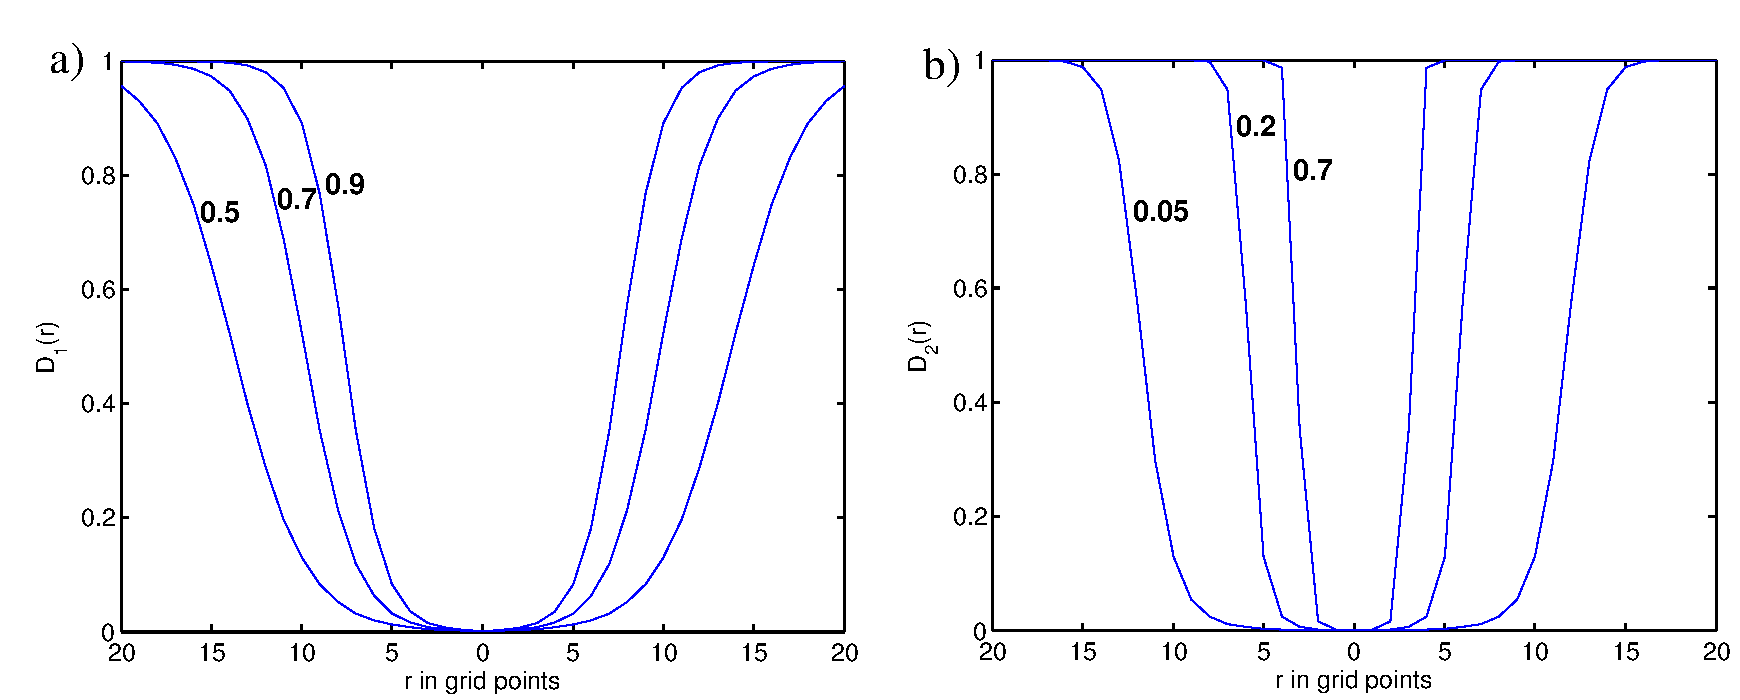
\includegraphics[width=0.8\textwidth]{fig/taper}
\caption[Exemplary taper functions for preconditioning]{Taper functions $D_1$ (a) $D_2$ (b)  with $a=1000$ for a source or receiver located at zero distance plotted for different values of $b$. }\label{fig:taper}
\end{figure}
Three types of local preconditioning are implemented in IFOS3D:\\
- a spherical tapering around source and receiver positions,\\
- a taper around source and receiver planes,  \\
- a taper of the C-PML boundaries\\
The tapering of the C-PML boundaries $D_{PML}(\textbf x)$ is implemented using the $D_2$-function, where the distance to the model boundary is used for $r$. It can be necessary because FWI tends to produce artefacts in the boundary. Using a source taper $D_s$ and a receiver taper $D_r$ the total preconditioned gradient can be estimated as 
\begin{equation} \textbf{p}_k(\textbf x)=D_sD_rD_{PML}\nabla E_k.\end{equation}

\section{Calculation of the conjugate gradient as search direction}
The preconditioned gradient can be used as search direction for updating the model as seen in equation~\ref{equ:update1}. However, the use of the conjugate gradient can stabilise the inversion and improve convergence. The preconditioned gradient of the current iteration ($\textbf p_k$) and the preconditioned gradient ($\textbf p_{k-1}$) and conjugate gradient ($\textbf c_{k-1}$) of the previous iteration are used to calculate the conjugate gradient direction according to the equations~\ref{equ:conjgrad1} and \ref{equ:beta}. Thus, the application of the conjugate gradient method requires the storage of preconditioned gradient and conjugate gradient of the previous iteration.\\
The conjugate gradient gives the direction for the model update, but does not contain information about its size (also with respect to other parameter classes). We therefore normalise  $\textbf c_{k}$ to its maximum and multiply it with a reference value of the respective parameter class ($v_p^0$, $v_s^0$, $\rho^0$): 
\begin{equation}
 c_k^{v_p}(\textbf x)\rightarrow\frac{c_k^{v_p}(\textbf x)}{max(c_k^{v_p}(\textbf x))}v_p^0 \hspace{0.8cm} c_k^{v_s}(\textbf x)\rightarrow\frac{c_k^{v_s}(\textbf x)}{max(c_k^{v_s}(\textbf x))}v_s^0  \hspace{0.8cm} c_k^{\rho}(\textbf x)\rightarrow\frac{c_k^{\rho}(\textbf x)}{max(c_k^{\rho}(\textbf x))}\rho^0 \label{equ:scaled_grad}
\end{equation}
Additionally, a step length estimation is performed as described in the next section.

\section{Step length calculation}\label{sec:steplength}
A good step length calculation is crucial for a good performance in FWI. However, run time for its estimation should be low. IFOS3D uses a parabola  method \citep[e.g.][]{Kur09} to find the optimal step length, which can be achieved at reasonable computational costs. Additionally to the current model misfit the misfit values for two test step lengths are calculated. To mitigate runtime, this is only done for a subset of shots ($N_s$(step)). The three misfit values are used to find a parabola. The location of its minimum is adopted as optimal steplength $\alpha_k$ for the  model update. This results in ($2\times N_s$(step)) additional forward modelings.\\
Of course, the parabola is only a rough approximation of the real misfit curve. Therefore additional condtitions are employed for a successfull steplength estimation:
\begin{enumerate}
 \item in case, the parabola extremum is a maximum, I use the test steplength with the smallest misfit
\item a maximum steplength is defined, which cannot be exceeded
\item if a steplength of zero is estimated or the steplength is negative, the model is updated using a small ratio of the first test-steplength
\end{enumerate}
The choice of the test step length is important for the performance of this method. Generally, the test step length can be larger at the beginning of the inversion, when larger model updates determine the rough structure of the subsurface. Later smaller changes of the model are required for the finer model structures. In IFOS3D an initial test step length (TESTSTEP) is chosen and employed in the first iteration within each frequency band. For later iterations the optimal steplength $\alpha_k$ of the previous iteration is used and the new test step length is determined as $\alpha_k/2$. If the new test step length is larger than TESTSTEP, TESTSTEP is used for the next iteration. If the new test step length is smaller than 25\% of TESTSTEP, it is set to 25\% TESTSTEP.\\
Note, that one steplength is estimated for all parameter classes. It can be useful to limit the update of one parameter class with respect to another. This can be achieved by applying weighting factors in the model update. 
\section{The model update} 
Starting from some starting model the model in each iteration $k$ is updated with $(-\alpha_k\textbf c_k)$.\\
In general, the elastic FWI updates three parameter classes ($v_p$, $v_s$ and $\rho$). The conjugate gradients are calculated for each parameter class and are scaled with an average of this parameter to take into account the size of these parameters with respect to ech other. However, note that only one step length is estimated for all parameters. It can be useful to limit the update of one parameter class with respect to another. This can be achieved by applying additional weighting factors in the model update. 
\section{The full inversion process}
Full waveform inversion is an iterative process. We search for the optimal model by updating the model parameters in the direction of the steepest descent of the misfit function to reach its minimum. However, the inversion of seismic data is generally highly nonlinear and the misfit function is not a smooth function, but contains a lot of local minima. Using a local inversion method like the conjugate gradient approach, it is possible to end up in a local minimum. In this case, the observed data might be explained relatively well by the inverted model, but the model structures are not correct. To find the real subsurface model, the choice of the starting model and different inversion strategies are important.
\subsection{The starting model}
The choice of the starting model is crucial for FWI. The starting model should contain preliminary information about the subsurface, especially for complex data. It can be useful to use a smooth starting model because hard contrasts of interfaces and structures are difficult to change with FWI. The starting model should already approximately explain the low frequency data so that no cycle skipping problems arise. This means, that the required smoothness of the starting model is dependent on the availability of low frequency data.
\subsection{Multi-scale inversion}
It is very helpful not to invert the whole data set at once, but to start with a portion of data and add more data in different stages of the inversion. There are generally three different types for the selection of data:
\begin{enumerate}
 \item frequency filtering: The inversion starts with the inversion of low frequency data and subsequently adds higher frequencies,
 \item time windowing: first arrivals are inverted as a first step, and more data is added in later stages,
 \item offset windowing: seperate long and short offset data
\end{enumerate}
The choice of the inversion strategy depends on the dataset and on the complexity of the problem and a combination of different strategies can be useful. In IFOS3D only the first strategy, the frequency filtering is available at the moment. In the following,
we will explain this method in more detail.
\subsection{Frequency stages}
\begin{figure}[h!]
\begin{center}
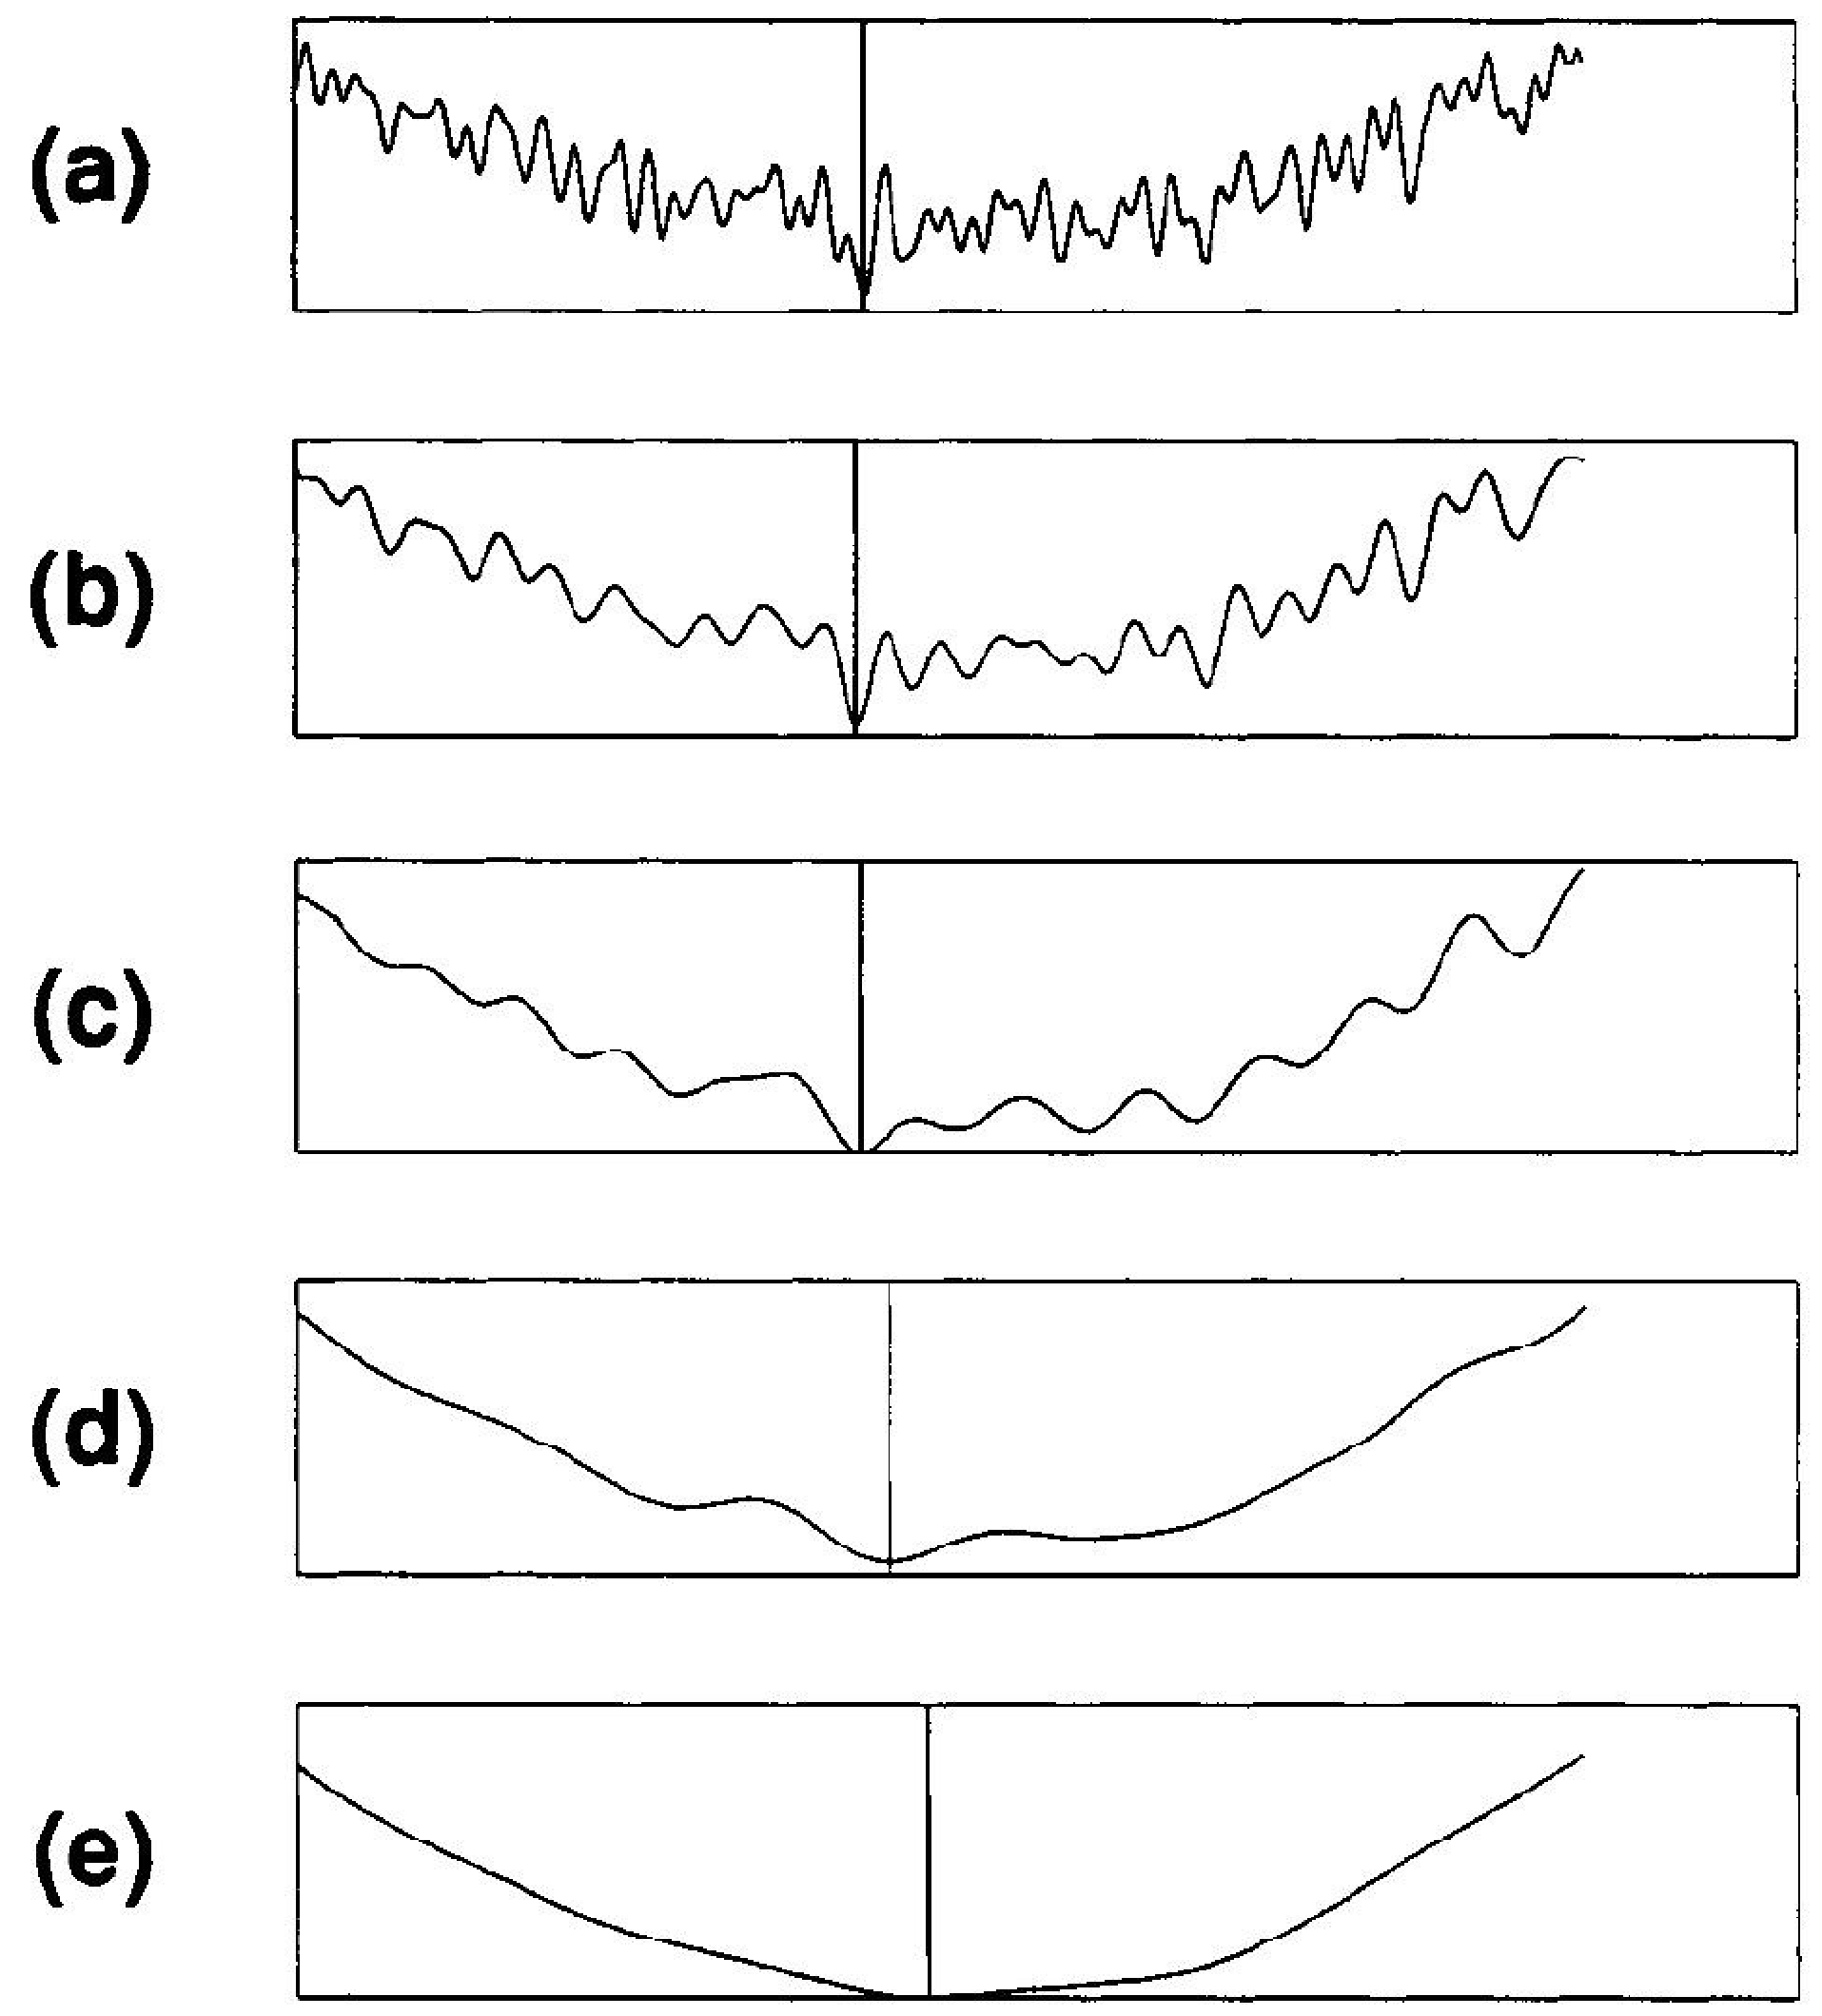
\includegraphics[width=0.5\textwidth]{fig/misfit_bunks}
\caption[Misfit at different scale lengths (from \cite{Bun95})]{Illustration of the misfit function for scale lengths increasing from a) to e) [from: \cite{Bun95}].}\label{fig:bunks}
\end{center}
\end{figure}
IFOS3D calculates the gradient from few monochromatic frequency domain wavefields. Hereby the inversion is subdivided into different frequency stages, which use a different set of frequencies. It is a common technique in FWI to start from low frequencies, to invert for the larger-scaled subsurface structures and then include higher frequencies to find finer model structures. This approach is well demonstrated by Figure~\ref{fig:bunks} from \citep{Bun95}. The misfit function is plotted for different scale lengths, which increase from a) to e). With increasing scale, and thus with decreasing frequency, the misfit function becomes smoother and the number of local minima decreases. Therefore, to reach the global minimum, a model can be much farther away from the real model for low frequencies, whereas a much closer model is required for high frequencies. This can also be understood when looking at the data. Phase differences between the modelled and the observed data need to be smaller than half a period, so that the phases can be assigned correctly to each other. Otherwise cycle skipping can occure and the inversion might end up in a local minimum. This condition is easier to fullfill for lower frequencies. Hence, a multi-scale approach in FWI can mitigate the problem of cycle-skipping and help to reach the global minimum.
\subsubsection*{The choice of frequencies}
There are different ways to include higher frequencies in a multi-scale inversion. \cite{Bro09} tested three different approaches:
\begin{itemize}
\item sequential approach: single frequency inversion using one frequency at a time
 \item Bunks approach: starting from one low frequency, one higher frequency per stage is added, so that the number of frequencies per stage increases
\item simultaneous approach: a group of typically 3-5 frequencies is inverted in each stage, overlapping frequency bands
\end{itemize}
Overall, they found the best performance for the simultaneous inversion of several frequencies, with overlapping frequency bands for their reflection geometry application. Thus, the entrainment of the lower, already inverted frequencies in the Bunks approach does not seem to improve the inversion. \cite{Pra99} also showed an improved performance, when using five instead of three frequencies during one frequency stage. Thus a higher number of frequencies can improve the inversion and a single frequency approach does not seem to be favourable, even though successful applications show that single frequency inversions are possible.\\
Fortunately, the use of frequency groups with few frequencies per stage instead of a single frequency in a time-frequency FWI does not increase the computational costs by much. By contrast when employing a frequency domain forward solver, these frequencies need to be simulated additionally.
\subsubsection*{Frequency intervals}
The choice of the frequency interval needs to ensure a continuous coverage of the wavenumber spectra. \cite{Sir04} showed, that this can generally be fulfilled for frequency intervals larger the sampling interval of $1/T$ ($T$: length of time series), when considering not only one trace but a range of offsets.  Hereby larger offsets enable the coverage of the wavenumber spectra with a lower frequency sampling. For a simple 1D model, the relevant frequencies can be calculated with 
\begin{equation} f_{n+1}=\frac{f_n}{\alpha_{min}},\end{equation}
where $\alpha_{min}$ depends on the offset-to-depth ratio and is smaller for larger maximum offsets \citep{Sir04}.  Still, the use of additional  frequencies increases the redundancy of the data which generally results in improved images, especially in case of higher nonlinearity of the inversion.
\section{Preconditioning with the diagonal Hessian approximation}\label{sec:hess}
In section~\ref{sec:preconditioning} we discussed a very simple method of preconditioning, which locally damps the gradient around sources and receivers. This method works nicely for simple problems as for example often found in transmission geometries. However, in case of complex wavefields this method is not sufficient. If we look at surface geometries, we find that the gradient is very concentrated near the surface, where most energy of the wavefield travels. This means that deeper model parts are not updated without an enhancement by preconditioning. IFOS3D offers the  possibility to employ an approximation of the diagonal Hessian for preconditioning. This approach takes information about the second derivative of the misfit function, the Hessian into account and is a physically funded method. The diagonal elements of the Hessian predict the geometrical amplitude spreading contained in the gradient and can thus be used  to find an improved  spatial scaling of the gradient. In surface seismic, the scaling of the gradient with the diagonal elements of $\textbf H_a$ enhances the influence of deeper parts of the model. In the following we will give an overview about the implementation. For additional information about the role of the Hessian in FWI we refer to \cite{Pra98, Vir09, Bro11} and \cite{But15}.
\subsection{The Hessian operator}
The full Newton method uses the Hessian marix $\textbf H$ for its model update given by
\begin{equation} \delta\textbf m=-\textbf H^{-1}\nabla_mE.\end{equation} In case of a linear inversion problem, an update with $\delta\textbf m$ would lead into the minimum of the misfit function within one step. Non-linear inversion problems, like FWI are linearised step-wise and iteratively approach the minimum. Still the convergence of the Newton method is much improved compared to the gradient methods.
The Hessian is the second derivative of the misfit function with respect to the model parameters:
\begin{equation}H_{jl}=\frac{\partial^2 E(\textbf m)}{\partial m_j\partial m_l} \hspace{0.5cm} (j=1,...n)\hspace{0.2cm}(l=1,...n). \label{equ:hessb}\end{equation}
The variable $n$ denotes the number of model parameters. The size of $\textbf H$ with $n\times n$ is huge and its explicit calculation is therefore very expensive. For large FWI problems like the 3D elastic FWI applications it is not possible. Still the gradient method can be improved by using some information about the Hessian. Comparing the model update of the gradient method (equation~\ref{equ:update1}) with the Newton update, the gradient method approximates $\textbf H$ by $\alpha \textbf P$. By preconditioning the gradient with an approximation of the diagonal Hessian it is thus possible to improve the gradient method.
\subsection{Theory}
\subsubsection*{Calculation of the diagonal Hessian approximation}
The second derivative of the $L_2$-norm based misfit function (equation~\ref{eq:L2}) can be expressed as   \begin{equation}H_{jl}=\sum_{s}\int_0^T dt \sum_{r}\frac{\partial u_i}{\partial m_j}\frac{\partial u_i}{\partial m_l}+R_{jl} =(H_a)_{jl}+R_{jl}.\label{equ:Hess_L2}\end{equation}
In the following we neglect the second term $R_{jl}$ which contains second order partial derivative wavefields and constrain to the first term, the so-called ``approximate Hessian'' $(H_a)_{jl}$. It is calculated as a zero-lag cross-correlation of the first order partial derivative wavefields summed up over all sources $s$ and receivers $r$.\\
For preconditoning in IFOS3D we only use the diagonal elements and calculate the elements $(H_a)_{jj}$ for discrete frequencies. Equation~\ref{equ:Hess_L2} then transforms to \citep{But15}
\begin{equation}(H_a)_{jj}=\sum_{s}\sum_{r}\sum_{v=1}^{nf}\frac{\partial\tilde u_i}{\partial m_j}\left(\frac{\partial\tilde u_i}{\partial m_j}\right )^*. \label{Hess_diag}\end{equation}
The adjoint gradient method does not directly calculate the partial derivative wavefields also known as Fr\'echet derivative kernels which are now required for the estimation of the elements $(H_a)_{jj}$. The derivatives with respect to the elastic parameters $\lambda$, $\mu$ and $\rho$ in frequency domain can be expressed as (see \cite{But15})
\begin{equation}
\begin{split}
 \frac{\partial \tilde u_i(\textbf x_r,\omega_v)}{\partial\rho(\textbf x)} & =\omega_v^2\tilde G_{ji}(\textbf x,\omega_v;\textbf x_r,0)\tilde u_j(\textbf x,\omega_v),\\
\frac{\partial\tilde u_i(\textbf x_r,\omega_v)}{\partial\lambda(\textbf x)} & =-\frac{\partial}{\partial x_j}\tilde G_{ji}(\textbf x,\omega_v;\textbf x_r,0)\frac{\partial\tilde u_p(\textbf x,\omega_v)}{\partial x_p},\\
\frac{\partial\tilde u_i(\textbf x_r,\omega_v)}{\partial\mu(\textbf x)} & =-\frac{1}{2}\left (\frac{\partial}{\partial x_k}\tilde G_{ji}(\textbf x,\omega_v;\textbf x_r,0)+\frac{\partial}{\partial x_j}\tilde G_{ki}(\textbf x,\omega_v;\textbf x_r,0)\right )\left (\frac{\partial\tilde u_j(\textbf x,\omega_v)}{\partial x_k}+\frac{\partial\tilde u_k(\textbf x,\omega_v)}{\partial x_j}\right ).
\end{split}\label{equ:frechet4}
\end{equation}
The terms $\tilde G_{ji}(\textbf x,\omega_v;\textbf x_r,0)$ denote the Green's receiver functions for discrete frequencies, which are multiplied with the forward wavefields. Same as for the gradient calculation we transform these equations to the seismic velocity parametrisation by using the chain rule
 \begin{equation}
\begin{split}
 \frac{\partial\tilde u_i}{\partial v_p}& =2\rho v_p\frac{\partial\tilde u_i}{\partial\lambda},
\\
\frac{\partial\tilde u_i}{\partial v_s}& = -4\rho v_s\frac{\partial\tilde u_i}{\partial\lambda}+2\rho v_s\frac{\partial\tilde u_i}{\partial\mu},
\\
\frac{\partial\tilde u_i}{\partial\rho'}& = (v_p^2-2v_s^2)\frac{\partial\tilde u_i}{\partial\lambda}+v_s^2\frac{\partial\tilde u_i}{\partial\mu}+\frac{\partial\tilde u_i}{\partial\rho}.
\end{split}\label{equ:partial_wave2}
\end{equation}
Finally these partial derivative wavefields can be used for the estimation of the diagonal Hessian approximation $H_a^{v_p}(\textbf x)$, $H_a^{v_s}(\textbf x)$ and $H_a^{\rho'}(\textbf x)$ (equation~\ref{Hess_diag}).
\subsubsection*{Hessian preconditioning}
As preconditioning operator ($P^\rho(\textbf x)$, $P^\lambda(\textbf x)$ and $P^\mu(\textbf x)$) for the different parameters we use the inverse of the diagonal of $\textbf H_a$, which is straightforward for a diagonal matrix:
\begin{equation}
 \begin{split}
 P^\rho(\textbf x) & = (H_a^\rho(\textbf x)+\epsilon_\rho)^{-1},\\
 P^{v_p}(\textbf x) & = (H_a^{v_p}(\textbf x)+\epsilon_{v_p})^{-1},\\
 P^{v_s}(\textbf x) & = (H_a^{v_s}(\textbf x)+\epsilon_{v_s})^{-1}.
\end{split}\label{Hess_precon}
\end{equation}
The coefficients $\epsilon_\rho$, $\epsilon_\lambda$ and $\epsilon_\mu$ are water levels, which are summed to the Hessian approximations for reasons of stability. Otherwise, very small elements of $\textbf H_a$ in areas of very low wave coverage cause a strong increase of the gradient in these areas which can result in artefacts.
\subsection{Implementation of Hessian preconditioning}
The implementation of Hessian preconditioning in IFOS3D is illustrated in figure~\ref{fig:workflow_hess}. Note, that the Hessian computation depends on the acqusition geometry and the current model $\textbf m_k$ but does not contain information about the true subsurface model.
\begin{figure}[h!]
\begin{center}
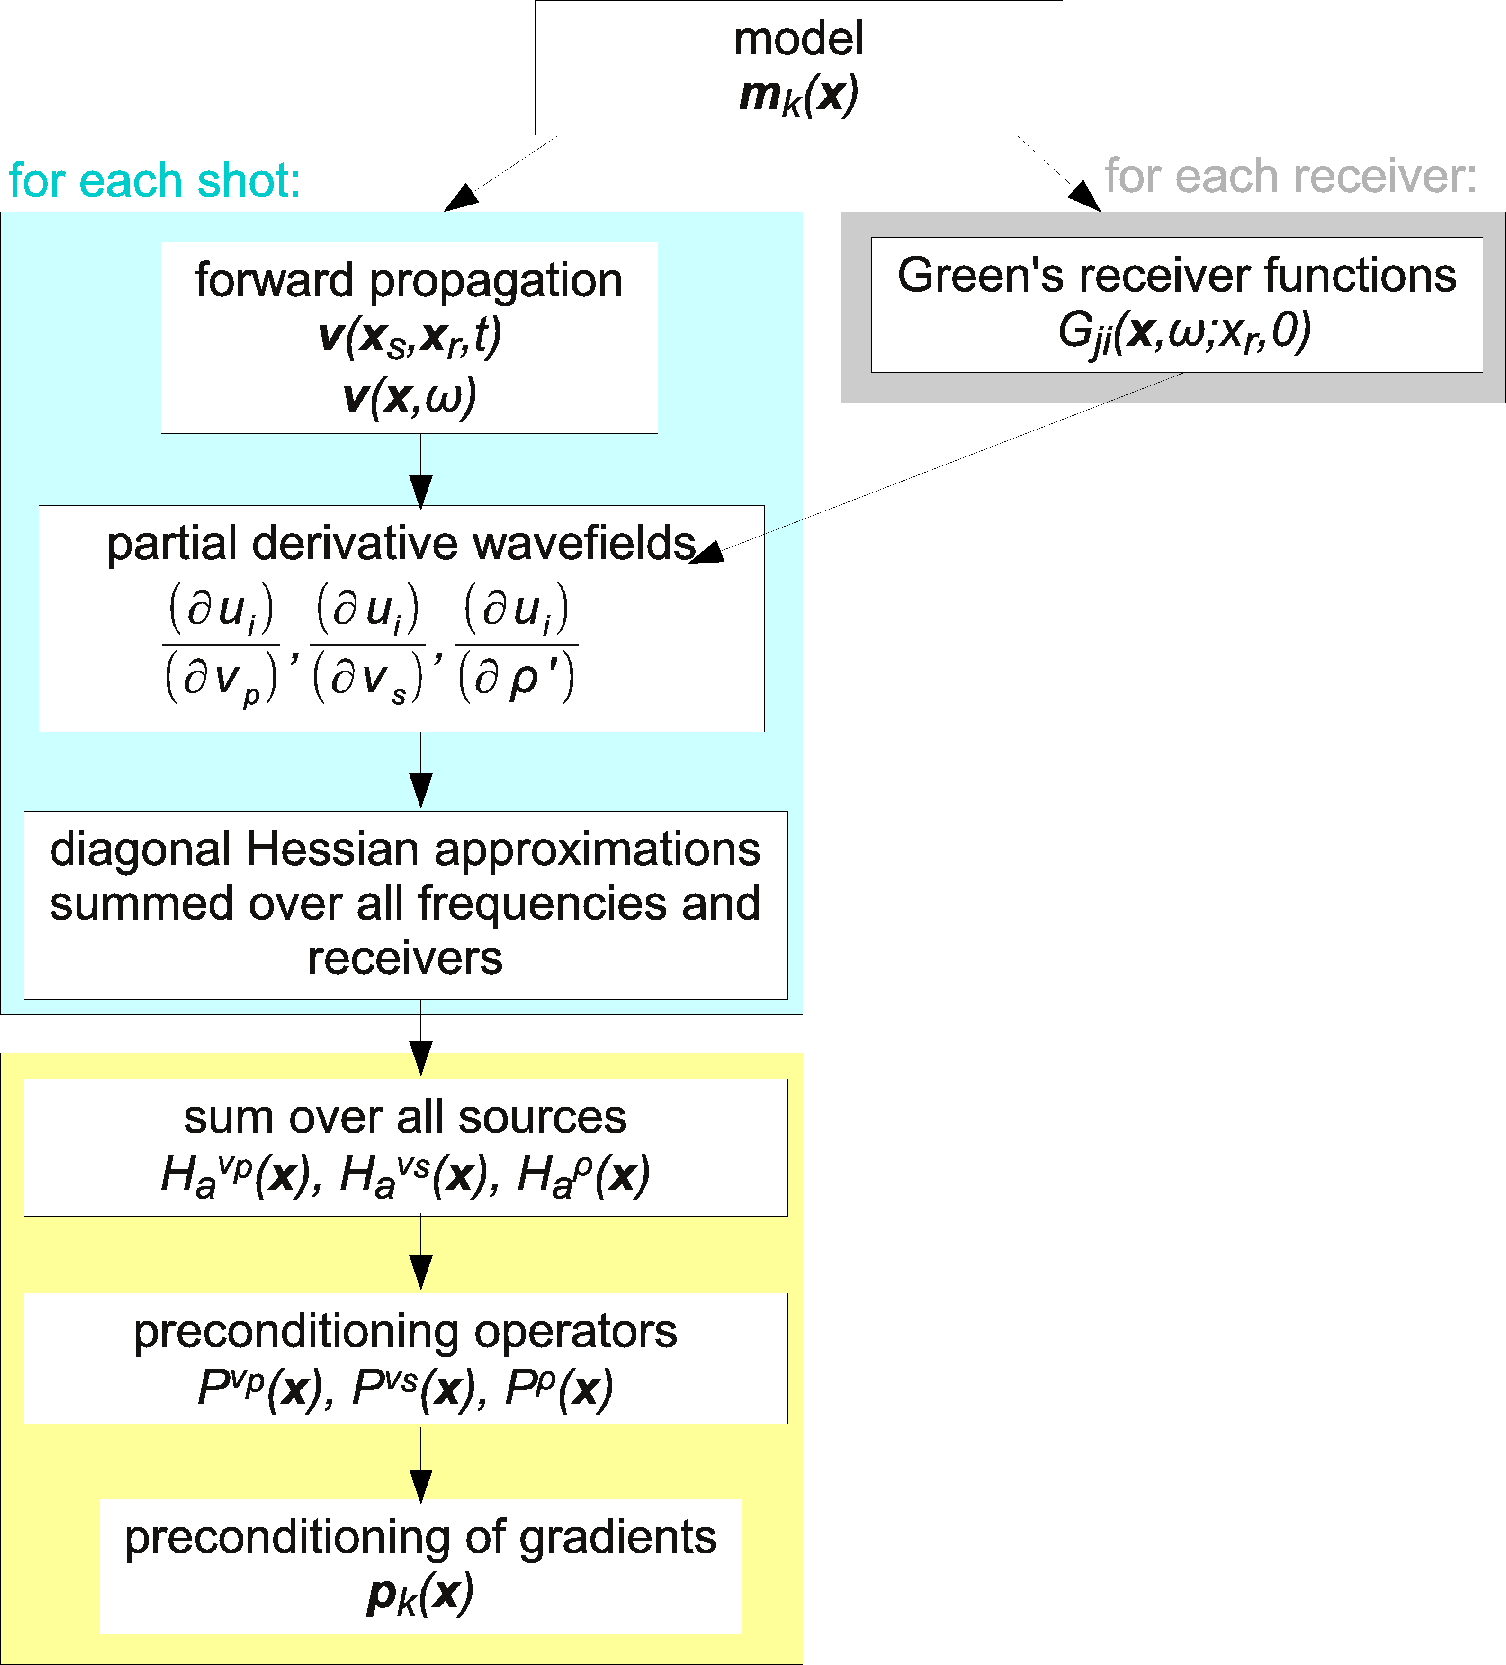
\includegraphics[width=0.75\textwidth]{fig/workflow_hess_22}
\caption[Workflow for the calculation of the Hessian preconditioning operator]{Workflow for the calculation of the Hessian preconditioning operator at iteration $k$ as implemented in IFOS3D.}\label{fig:workflow_hess}
\end{center}
\end{figure}
\subsubsection*{Wavefield calculation}
The forward propagation of wavefields and the extraction of monochromatic frequency wavefields ($\textbf v(\textbf x,\omega$)) is already performed in the framework of the gradient calculation (section~\ref{sec:grad_calc}). The main additional computational effort is spend for the computation of the Green's receiver functions $\tilde G_{ji}(\textbf x,\omega_v;\textbf x_r,0)$. Differently to the gradient calculation, where the backpropagated wavefield is propagated from all receivers simultanously, the complete set of Green's receiver functions requires one propagation for each receiver and each component, resulting in $3\times N_{rec}$ additional wavefield simulations ($N_{rec}$: total number of receivers). We calculate the Green's receiver functions for displacement by using a Heaviside step function ($\Theta$) as a force-time function, defined as 
$$\Theta(t-t_{step})=
 \begin{cases}
  0 \mbox{ for } t<t_{step}\\
1\mbox{ for } t\geq t_{step},
 \end{cases}$$
with the $\delta(t-t_{step})$-function as its derivative. The same time shift $t_{step}$ is used for the forward source. To estimate the Green's receiver functions in frequency domain, we apply a discrete Fourier transform (equation~\ref{equ:discFourier}) to the function $G_{ij}(\textbf x_r,t;\textbf x,t_{step})$ on the fly. The functions $G_{ij}(\textbf x_r,\omega_v;\textbf x,0)$ are stored in memory for each discrete frequency and each receiver. Due to the high computational runtime and storage demand, we employ two approximations here. Firstly, we only use a subset of receivers. Secondly, we only calculate the component of the Green's receiver functions which corresponds to the source of the forward wavefield and thus calculate only one component of the partial derivative wavefield. These limitations have only small effects on the gradient corrections near the source, where preconditioning is most important. However, an additional local preconditioning of the smaller receiver artefacts becomes necessary. 
\subsubsection*{Hessian calculation}
For each shot the partial derivative wavefields are computed by multiplying the forward field with each Green's receiver function for each frequency according to equations~\ref{equ:frechet4} and \ref{equ:partial_wave2}. Hereby, the velocities of the forward wavefield are integrated with $(i\omega)^{-1}$ to find the displacement fields and spatial derivatives are calculated with finite differences of fourth order. The partial derivative wavefields are multiplied with their complex conjugate and summed up over all frequencies and receivers and finally over all shots to find the diagonal Hessian approximation for $v_p$, $v_s$ and $\rho$ (equation~\ref{Hess_diag}). 
\subsubsection*{Preconditioning}
Finally, the preconditioning operator can be calculated according to equation~\ref{Hess_precon} and applied to the gradient ($\textbf P(\textbf x) \nabla E_k$). At the moment no automatic estimation of the water levels $\epsilon$ is implemented and the water levels are taken from the input file. Thus an empirical try of $\epsilon$ and its effects on the gradient preconditioning is required using the gradient and Hessian of the current iteration.\\
An additional local damping of the gradient around the receiver positions and in the C-PML boundaries is applied.
\subsubsection*{The full inversion process}
The Hessian preconditioning operator is calculated once at the beginning of each frequency stage. It is applied throughout this stage. Unfortunately, the estimation of the water level $\epsilon$ is not automised at the moment. That means, that in practice before the inversion starts a new frequency stage, the gradient and Hessian are estimated and the water level is determined empirically. This results in as additional calculation of the first gradient of each frequency stage.\\
Apart from the calculation and application of the Hessian preconditioning operator the inversion process, like gradient normalisation, model update and steplength calculation remains unchanged. 
\subsubsection*{Costs of Hessian preconditioning}
The Hessian preconditioning operator is calculated once per frequency stage. The main extra run time is spend for the modelings of the Green's receiver functions which number corresponds to the subset of receivers used for these calculations. Additionally, one extra gradient computation is performed as long as the empirical determination of $\epsilon$ before each frequency stage is required.\\
In summary, the following approximations are made compared to the use of the full Hessian matrix:
\begin{itemize}
 \item use of diagonal elements of $\textbf H_a$ only,
\item employ only a subset of receivers for its calculation,
\item only one component of partial derivative wavefields by  backpropagating only one component $\delta$-pulse and
\item estimate Hessian only once for each frequency stage.
\end{itemize}

\section{The L-BFGS method}\label{sec:lbfgs}
This section introduces the L-BFGS (low memory BFGS) method, named after the BFGS-method developers, i.e. Broyden, Fletcher, Goldfarb and Shannon. The method belongs to the class of the quasi-Newton methods and is implemented in IFOS3D as an optimisation of the inversion process. The Hessian operator and Newton methods were shortly explained in the previous chapter. Instead of calculating the inverse Hessian $\textbf H_k^{-1}$ directly, quasi-Newton methods approximate the (inverse) Hessian by using the change of the gradients over the iterations. Starting from an initial Hessian approximation $\textbf H_0$ the approximation of the (inverse) Hessian is updated in each iteration to find a more accurate estimate for the Hessian. \\
The application of the inverse Hessian to the gradient acts as deconvolution of the gradient from limited-bandwidth effects and geometric amplitude effects \citep{Pra98,Bro09}. Previous applications for 2D FWI by \cite{Bro09} and \cite{Bro11} showed higher convergence rates and sharper images when using the L-BFGS approach compared to the conventional conjugate gradient method. Additionally, a correct inversion of multiple parameter classes can be achieved which requires no empirical weighting of the different parameter classes.
\subsection{Theory of the BFGS and L-BFGS method}
Using the changes of the gradients $\pmb{\gamma}_k=\nabla E_{k+1}-\nabla E_{k}$ and the model changes $\textbf s_k=\textbf{m}_{k+1}-\textbf{m}_{k}$ the BFGS-condition is formulated as \citep{Noc99}
\begin{equation}
 \textbf{H}_{k+1}^{-1}=\textbf V_k^T\textbf H_k^{-1}\textbf V_k+r_k\textbf s_k\textbf s_k^T \hspace{0.5cm} \text{with} \hspace{0.2cm} r_k=\frac{1}{\pmb{\gamma}_k^T\textbf s_k}  \hspace{0.5cm} \text{and} \hspace{0.2cm}\textbf V_k=\textbf I-r_k\pmb{\gamma}_k\textbf s_k^T.\label{equ:BFGS}
\end{equation}
The inverse Hessian approximation is updated in each iteration starting from an initial guess $\textbf H_0^{-1}$ without explicitely calculating the second derivatives. However, it is not suitable for a large number $n$ of model parameters due to the huge size of the Hessian matrix ($n\times n$).\\
By contrast, the L-BFGS method does not explicitely store the Hessian matrix, but uses changes in gradient and model of only the recent $m$ iterations and calculates the inverse Hessian newly in each iteration. Applying equation~\ref{equ:BFGS} repeatedly for the previous $m$ iterations results in the following formula \citep{Noc99}:
\begin{equation}
 \begin{split}
  \textbf H_k^{-1}=& (\textbf V_{k-1}^T...\textbf V_{k-m}^T)\textbf H_{k0}^{-1}(\textbf V_{k-m}...\textbf V_{k-1})\\
      & +r_{k-m}(\textbf V_{k-1}^T...\textbf V_{k-m+1}^T)\textbf s_{k-m}\textbf s_{k-m}^T(\textbf V_{k-m+1}...\textbf V_{k-1})\\
      & +r_{k-m+1}(\textbf V_{k-1}^T...\textbf V_{k-m+2}^T)\textbf s_{k-m+1}\textbf s_{k-m+1}^T(\textbf V_{k-m+2}...\textbf V_{k-1})\\
      & +... \\
      & +r_{k-1}\textbf s_{k-1}\textbf s_{k-1}^T.
 \end{split}\label{equ:LBFGS}
\end{equation}
$\textbf H_{k0}^{-1}$ is an initial inverse Hessian approximation, which is allowed to vary from iteration to iteration.
\subsection{The L-BFGS update}
The L-BFGS method can be implemented very efficiently in FWI. In IFOS3D we apply the recursive algorithm described by \cite{Noc99} which estimates the product $\textbf H_k^{-1}\nabla E_k$ without forming the inverse Hessian approximation directly. It can be written as \vspace{0.5cm}\\
\line(1,0){125}\\
$\textbf q \leftarrow \nabla E_k$\\
\textbf{for} ($i=k-1,...,k-m$)\\
$\hspace*{1cm} \alpha_i \leftarrow r_i\textbf s_i^T\textbf q$\\
\hspace*{1cm} $\textbf q\leftarrow\textbf q-\alpha_i\pmb{\gamma}_i$\\
\textbf{end for}\\
$\textbf z \leftarrow \textbf H_{k0}^{-1}\textbf q$\\
\textbf{for} ($i=k-m,...k-1$)\\
\hspace*{1cm}$\beta\leftarrow r_i\pmb{\gamma}_i^T\textbf z$\\
\hspace*{1cm}$\textbf z\leftarrow\textbf z+\textbf s_i(\alpha_i-\beta)$\\
\textbf{end for}\\
$\textbf H_k^{-1}\nabla E_k=\textbf z$\\
\line(1,0){125}\vspace{0.5cm}\\
This algorithm is performed once in each iteration and consists of $(4mn+n)$ multiplications if a diagonal $\textbf H_{k0}^{-1}$ is chosen. The L-BFGS algorithm requires additional storage of $(2mn+m)$ floating numbers for $\pmb\gamma, \textbf s$ and $r$. For reasonable numbers of $m$ the L-BFGS method can therefore be performed at relatively low extra costs of runtime an storage. In general, values between 5 and 20 are used for $m$. In the first $(m-1)$ iterations the result corresponds to the BFGS method. 
\subsection{The optimised FWI workflow}
\subsubsection{Hessian preconditioning and L-BFGS}
Following the approach by \cite{Bro11} we apply the L-BFGS method by using changes in gradients preconditioned by the diagonal Hessian approximation. The Hessian preconditioning (section~\ref{sec:hess}) already offers an improved scaling of the gradient. By additionally using the L-BFGS algorithm, the off-diagonal elements of the gradient are taken into account. Furthermore, the L-BFGS method is calculated in each iteration, whereas the diagonal Hessian matrix is estimated only once per frequency stage. When using the preconditioned gradients a scaled identity matrix \citep{Noc99} is sufficient as initial guess for the Hessian:
\begin{equation} \textbf H_{k0}^{-1}=\frac{\textbf s_{k-1}^T\pmb{\gamma}_{k-1}}{\pmb{\gamma}_{k-1}\pmb{\gamma}_{k-1}^T}\textbf I,  \end{equation}
\subsubsection*{Parameter normalisation}
The conjugate gradient does not offer information about the update of the different model parameters with respect to each other. This is changed when taking the off-diagonal elements of the Hessian into account. The L-BFGS method can thus improve the multi-parameter inversion by adding information about off-diagonal elements of the Hessian. To achieve a dimensionless L-BFGS sheme for the different parameter classes we normalise the inversion sheme with some representative model parameters $v_{p0}, v_{s0}$ and $\rho_{0}$ as suggested by \cite{Bro11} with   
\begin{equation}
 \hat v_p(\textbf x)=\frac{v_p(\textbf x)}{v_{p0}}, \hspace{0.5cm}\hat v_s(\textbf x)=\frac{v_s(\textbf x)}{v_{s0}}, \hspace{0.5cm}\hat \rho(\textbf x)=\frac{\rho(\textbf x)}{\rho_{0}}. 
\end{equation}
This leads to a normalisation of the gradients calculated as
\begin{equation}
 \frac{\partial E}{\partial\hat v_p(\textbf x)}=\frac{\partial E}{\partial v_p(\textbf x)}v_{p0},\hspace{0.8cm}\frac{\partial E}{\partial\hat v_s(\textbf x)}=\frac{\partial E}{\partial v_s(\textbf x)}v_{s0},\hspace{0.8cm}\frac{\partial E}{\partial\hat\rho(\textbf x)}=\frac{\partial E}{\partial \rho(\textbf x)}\rho_0
\end{equation}
and a normalisation of the Hessian approximation given by
\begin{equation}
 H_a^{\hat v_p}=H_a^{v_p}v_{p0}^2, \hspace{0.8cm} H_a^{\hat v_p}=H_a^{v_p}v_{p0}^2, \hspace{0.8cm} H_a^{\hat \rho}=H_a^{\rho}\rho_0^2.
\end{equation}
The L-BFGS algorithm calculates a normalised model update, which needs to be denormalised by multiplication with the representative model parameters:
\begin{equation}
\delta v_p=\delta\hat v_p v_{p0}, \hspace{0.8cm} \delta v_s=\delta\hat v_s v_{s0}, \hspace{0.8cm} \delta\rho=\delta\hat\rho\rho_0.
\end{equation}
This dimensionless inversion sheme enables a simultanous L-BFGS algorithm for all parameter classes.
\subsubsection*{Workflow overview}
The workflow of the optimised FWI inversion can be described as follows:\vspace{0.5cm}\\
\line(1,0){125}\\
\textbf{for each frequency stage}
\begin{itemize}
 \item calculate diagonal Hessian approximation ($H_a^{\hat v_p}, H_a^{\hat v_s}, H_a^{\hat\rho}$) for normalised parameters
\end{itemize}
\textbf{in each iteration}
\begin{itemize}
\item calculate gradients of normalised parameters
\item apply diagonal Hessian approximation to gradient 
\item save change in preconditioned gradients and models, discard iterations smaller k-m
\item L-BFGS algorithm to find normalised model update
\item denormalise model update
\item step length calculation: try steplength $\alpha=1$ first
\item model update
\end{itemize}
\line(1,0){125}\\
Newton methods in general calculate an absolute model update and for a linearised Newton method steplenghts close to one are expected. This is also the case for the quasi-Newton L-BFGS sheme. If a good approximation of the Hessian can be achieved  a steplength close to one will be favourable. It is possible to apply a steplength estimation as described in section~\ref{sec:steplength} with a test step length of 0.5 and 1. If the L-BFGS sheme works well, a steplength close to 1 will be estimated after a few iterations. Note, that in the first iteration the inversion corresponds to a gradient method with Hessian preconditioning.

